\section{现象、概念、数学和技术}

1.

想和大家解释一下什么是物理。

物理学的研究总是从现象出发。所谓现象就是人能真切、稳定、连贯地感受到的信息。

这些信息中有两类特别重要,一个是视觉、另外一个是听觉。

视觉和形有关,我们能真切地感受到物体的位置、形状、颜色等都是人视觉器官的本领。这些本领是人的生物性决定的,我们天生就有这样的本领。触觉也和形有关,视觉是可见的形,触觉则是可以触摸的形,触觉和视觉一样微妙,比如我们的手有发达的神经末梢,能够分辨出丝绸和铁块质地的区别,乃至更加精细,比如水和牛奶的区别。

可以说是视觉和触觉一起给了我们形的概念,给了我们关于空间的概念。概念是帮助我们下判断的,当我们说某物在上面、某物在下面的时候,就已经在下判断了。

我们可以沉浸在现象中,一言不发,一个人享受神经的冲动。我们不需要说出来,也不需要对自己或对别人做出肯定或否定的动作。

2.

概念用来下判断,下判断、肯定或否定式的做陈述是人社会化生存所必须的。人不是野兽,人总生活在人群中,人群中的个体需要交流,并且是点对点的交流,P2P,并形成结构和网络。

人群需要交流,我们利用声音现象来做这个事情。和视觉一样,人天生具有发声器官,能发出复杂的声音(不同音高、响度、音长等等),并有非常灵敏的听觉器官,能够感知20-2万赫兹频率的声波。

严格说,我们利用视觉也可以交流信息,但视觉利用的是光信号,可见光的波长是微米数量级的,这个长度和人本身的尺寸比太小了,在人生活的世界里,人所打交道的器物、建筑等都是和人尺寸相同的,光波比这个数字小太多,光波的波动性在人的世界里是体现不出来的。

波长是$\lambda$的波动能绕开尺度同是$\lambda$的障碍物,如果我们仔细观察水波碰到障碍物时的行为,就会同意我的这个说法。现在光波波长太小了,就相当于水波碰到一个巨大的障碍物,水波将继续前进,绕不到巨大障碍物的后面去。

现在则是光波波长比人世界中随便一个物件都小太多了,这意味着随便一个物件就能挡住光信号。可以设想一个人冲着我打手势,只要中间插进一个人,我就看不见了。这是为什么我们不用光信号进行人与人之间信息交流的原因。

声波的波长比较长,而且正好和人的尺度一个数量级,声音信号会有效地绕到尺寸是1米数量级物体的后面去。这样我们在教室外大喊一声,我们在教室里也能听到了。

3.

我们借用声音现象进行交流,就是语言了。语言里有很多概念。概念就是对我们感受到的现象、经验和情绪进行恰当的分类,分类并命名。

“红色”可以说是一个以视觉经验为基础的概念,我说拿给我一个红苹果,你拿给我一个青苹果,我不接,然后你拿了个红苹果给我,我接了并吃掉它。

这就是维特根斯坦所说的语言游戏,我要红苹果是基于我的视觉经验的,但我对红的经验没法替换你对红的经验,但我却可通过人和人的互动,使“Hong”这个声音对我们两个人都有意义。这个游戏还可以继续玩下去,我可以继续要“红砖头”,“红土”,“红木”等。类似地,我还可以管你要一杯热水,热的食物,乃至热情的拥抱。……

“热”或“红”就是概念,我们总是否定了一些,才能肯定何者为“红”,何者为“敷衍了事”的拥抱。这就已经是分类了,分类并命名之。这些类在人与人的互动中自然呈现。

如何分类?好的分类标准是什么?

较真的话自然是不重复,也不遗漏的分类标准。但实际上我们很难做到,甚至是不可能做到的,现象、经验总是拒绝被穷尽的。

我们奉行的是够用就行的实用主义标准,这个标准能贯彻的前提是人要有事情做,当然不一定是功利意义下的事情,也可以是纯游戏,纯娱乐。能持续、稳定地玩下去,自然就会有合用的标准,而且伴随着这样的生活,这样的游戏、分类会越来越精细,我们相互间可下越来越精细的判断。

比如慷慨和挥霍的区别是什么呢?勇敢和鲁莽的区别又是什么呢?

如果你不生活在特定的生活中,或你不曾玩儿那特定的游戏,你就不会做如此精细的判断。也没必要。

4.

人是一种惧怕变化的动物。但变化、不确定正是人间的生活。

春种秋收是天地规定的,这个是可以很靠谱的,但春天的某个下午我出门碰见了某个人,然后摔了个跟头则是完全不可预期的。

对确定的事物,我们总是充满好奇。对人而言昼夜更替,春夏秋冬是完全确定的现象,而且它们是人间生活的基本前提。天与地相对,天是绝对的神圣,永不朽坏,天上的星星以庄严的步伐不快也不慢地划过天空,而地则是不确定的,周期性的朽坏和重新萌发。

天的运行就是天文学,人最早在天象的观察中感受到绝对的规律,和绝对的可以依靠。但天象的周期太长了,几十年、几百年、甚至上千年,这里假设了一个循环的时间观,即天象可以用各种周期描述,各种周期之间的比例又都是简单的整数比,所以迟早所有的天象可以循环重复,只是因为各种周期太多,比例虽然都是整数比,但还是繁复,导致最终的周期是很大的一个数,比如柏拉图的大年就是3万6千年。

但无论如何我们已经有了一个以数学为基础的对天文学进行研究的纲领,即长时间地、持续地对天象进行观测,用数字记录天体在天空中的方位等等。

这件事对人来说是充满神圣感的,因为人要生存基本前提就是天一定会以确定的方式运行,昼夜更替,春夏秋冬。

持续地观察天体的运行,并一代代记录下来就成了一项伟大的事业,是“天人感应”,“天子是天在人间的代表”,“天子是天人中介”等一系列说法的前提。

5.

一代代持续地观天需要一系列技术的支撑:

(1)职业的僧侣或巫师,他们脱离生产,专门学习记录和推演的方法。(2)合适的文字或算术技术,比如——把一个完整的圆弧划分为360度,1度是60分,1分是60秒——就是合适的。(3)大型天文观测站和天文仪器,比如托勒密曾在《至大论》中曾描述了柱基、子午浑仪和赤道经纬仪等仪器。

6.

天文学的研究在古希腊的时候经历了一次范式转换,即由算术式的,纯记录式的研究转变为基于几何直观的,和机械模仿的研究方式。

这当然要归功于伟大的柏拉图学派。

一代代地记录天象,并编纂成泥板书是令人尊敬的,并且也积累了足够的定量的数据。而且这已经具有近代科学的特征了,今天的科学是从实验出发的,从实验数据出发,实验数据不是第一手的现象,它是从实验仪器中被批量生产出来的“实验事实”。

我们从实验数据出发,构造模型算法,通过模型算法计算理论值,然后再把理论值与实验数据进行比对。

柏拉图构造的是“几何-机械”式的模型,假想自己是造物主,给出天球的设计,并用立体几何的语言予以陈述。水星、太阳、月球、金星、火星、木星、土星、恒星各有各的天球,大小不一,都围绕着地球构成一个转速各不相同的几何体系。

利用几何学知识,和一些可以接受的假设,我们能估算地球的大小、月球的大小、太阳的大小、地球-太阳的距离,和地球-月球的距离等。我们也知道各天球围绕地球运行的周期,甚至看上去颇为古怪的“火星逆行”。

首先我们需要用恰当的几何语言去描述它们,其次我们要去解释它们,为什么天要如此安排呢?难道这一切都是凑巧。

7.

柏拉图学派的“几何-机械”范式是对僧侣世袭观天迷集团的“算术-簿记”范式的超越。但“几何-机械”范式的优越性并不体现在提供了更精确的理论值,或更小的理论-观测误差。

“几何-机械”范式的优越性是突破了对现象的束缚,它的趣味在于追求形式的优美,它研究的是符合“几何-机械”模型的宇宙,而非现实的宇宙,即被观天迷们仔细记录过并可利用内插-外推算法可精确预言日食月食的那个宇宙。

希腊-罗马的政客和哲学家们研习天文学,也并非是为了获得关于天的完整知识,而仅仅是为了获得一种智力的训练,天文学和算术、几何学一起成为古代精英教育的一部分。

理想或优美的形式提供了人模仿的摹本。人可通过模仿理想的天在地上构建人的秩序,也可通过合适的材料,比如青铜来模仿几何,这就是机械。古代的机械大师,从阿基米德到维特鲁威都是精于几何,熟知天文的。

8.

物理学家研究理想的形式,经典力学、量子力学都是形式的构建。经典力学研究的对象是质点、刚体、连续介质和那些可以还原为质点、刚体和连续介质的复杂体系。量子力学研究如何对一个体系量子化,有些可以量子化的对象——比如自旋——并没有经典对应,同时有些经典体系——比如引力——尚无一个可行的量子化方案。

我们总是从实验数据出发,并把理论计算值与实验数据进行比对,但比对并不意味着一定要对上,对不上也没有关系。如果天并不真的按照柏拉图学派设计的方式运行,但只要我们发现了这个形式,这个形式就有潜在的用途,或者我们可以用机械制造出这样一台天球仪,我们的天球仪是可以很好地被这个“几何”模型描述的。

9.

对形式的追求,对形式美的追求在物理学中是很重要的。“几何-机械”范式就是一种比“算术-簿记”范式更优美、更简洁的对天的表述。这意味着我们更容易理解柏拉图的宇宙,容易理解就意味着容易想象,更容易基于柏拉图的宇宙进行思维,几何式的直观是算术所无法企及的。

获得直观性,使越来越复杂精巧的物理计算变得重新可以想象和思维是非常重要的,想象和思维永远比计算更重要。在量子力学中狄拉克记号、路径积分、费曼图等都是很好的例子。

\begin{figure}[htbp]
\begin{center}
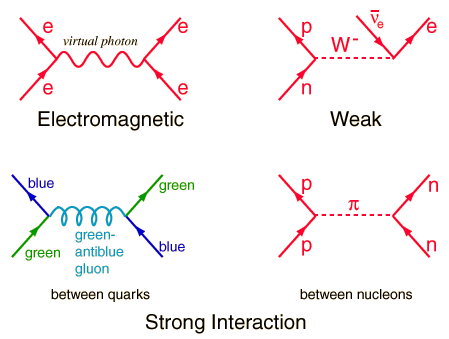
\includegraphics[width=10cm]{Appendix/feynmandiagram.png}
\caption{传说中的费曼图}
%\label{default}
\end{center}
\end{figure}

重新获得想象和思维的好处是我们可以主动地设计物理对象,就像我们可以做出天球仪一样,我们可以对材料进行设计,“制造”出自然界中并不存在的磁单极子等等。

对物理学家而言,像造物主一样去“造”远比“拯救现象”更激动人心。

%和追求理想相比,与现实符合算个屁!


~~

(这也是我设想的前言,呵呵,但还是放在后面吧。)

原始网址:\url{http://jianshu.io/p/c2a89d06f8bc}

%\newpage

\section{结束语}

如果有兴趣,大家还可继续阅读以下相关书籍:

\begin{enumerate}
\item 

J J Sakurai, Modern Quantum Mechanics

\item

格里菲思,《量子力学概论》(翻译或英文版)

\item

费曼,《费曼物理学讲义》(第三卷)

\end{enumerate}

或经常看看这个网站:PhysicsWorld,权威、全面而且通俗的物理网站(英文)。

\url{http://physicsworld.com/}

~~

2013-5-13
